\section{AAR Code Reference}

Selecting "AAR Codes" from the navigation drawer opens the Association of American Railroads (AAR) designation reference view. This page provides a standardized lookup table for rolling stock classification codes used throughout the inventory system, displaying the AAR Code, Rollingstock Type (RS Type), standard Description, and Action controls. Figure \ref{fig:aar} illustrates the main AAR Codes reference table.

\begin{figure}[H]
    \centering
    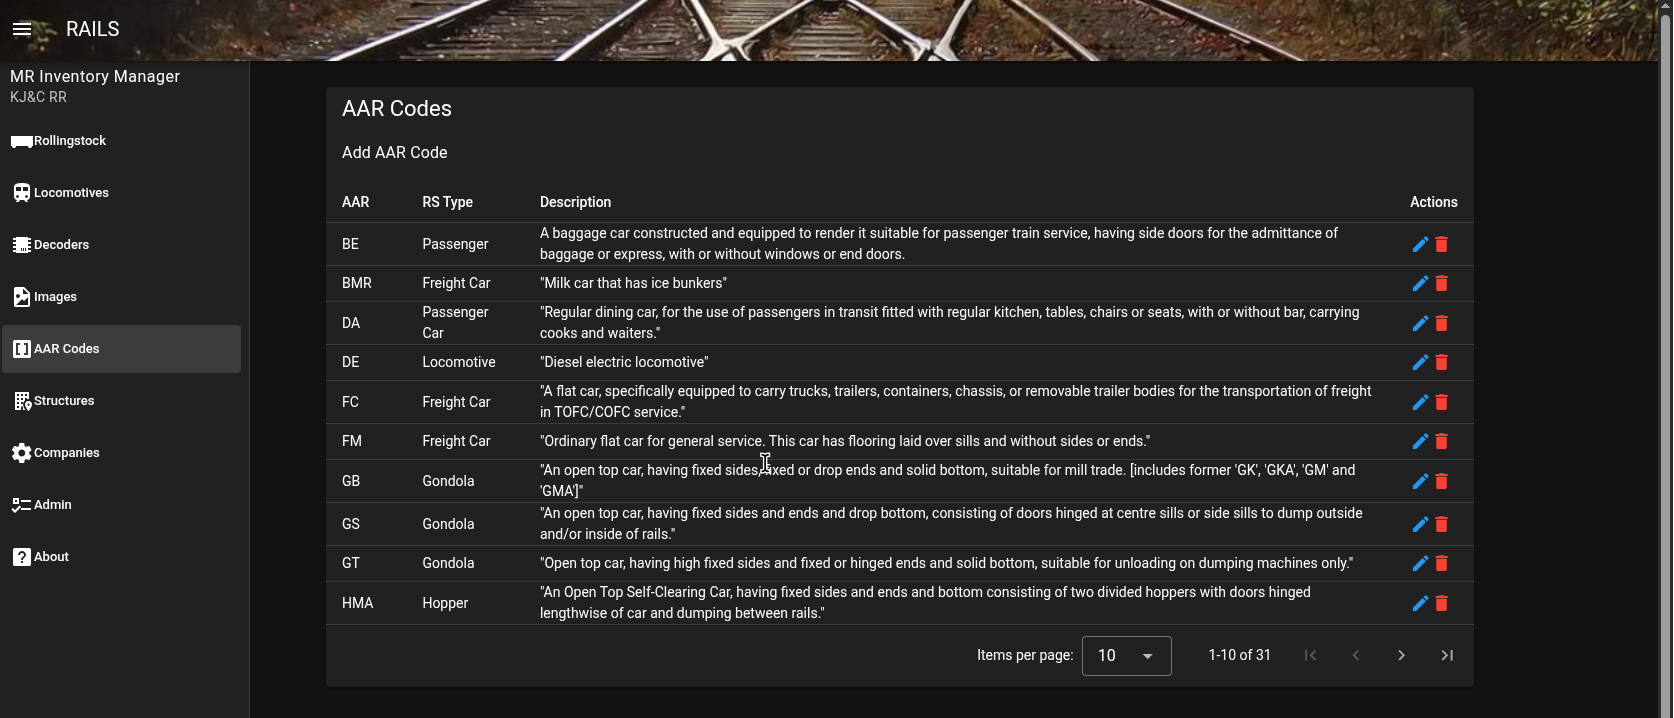
\includegraphics[width=0.85\textwidth]{./images/aar.png}
    \caption{AAR Codes Page}
    \label{fig:aar}
\end{figure}

\subsection{Adding an AAR Code}

Clicking the "Add AAR Code" button above the table opens a modal dialog to define a new equipment classification code. The form requires an AAR Code abbreviation, the associated RS Type, and a comprehensive Description detailing prototype car characteristics. Figure \ref{fig:aar-new} shows the entry modal.

\begin{figure}[H]
    \centering
    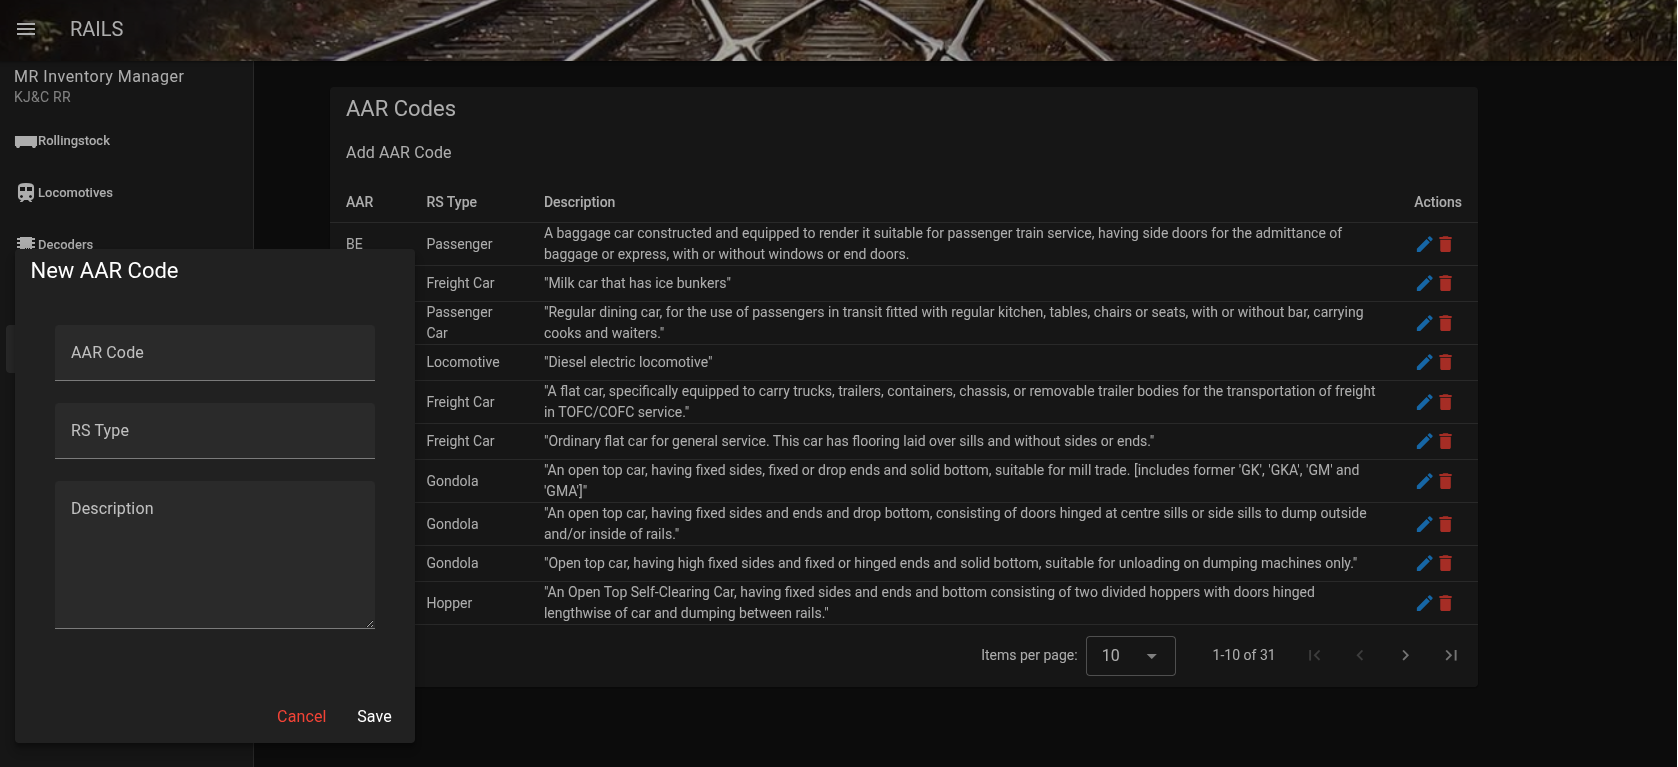
\includegraphics[width=0.85\textwidth]{./images/aar-new.png}
    \caption{Add AAR Code Dialog}
    \label{fig:aar-new}
\end{figure}

\subsection{Editing AAR Codes}

To modify an existing classification entry or update its prototype definition, click the blue pencil icon under the Actions column. This displays the AAR Code form with populated values for editing. Figure \ref{fig:aar-edit} shows the edit dialog interface.

\begin{figure}[H]
    \centering
    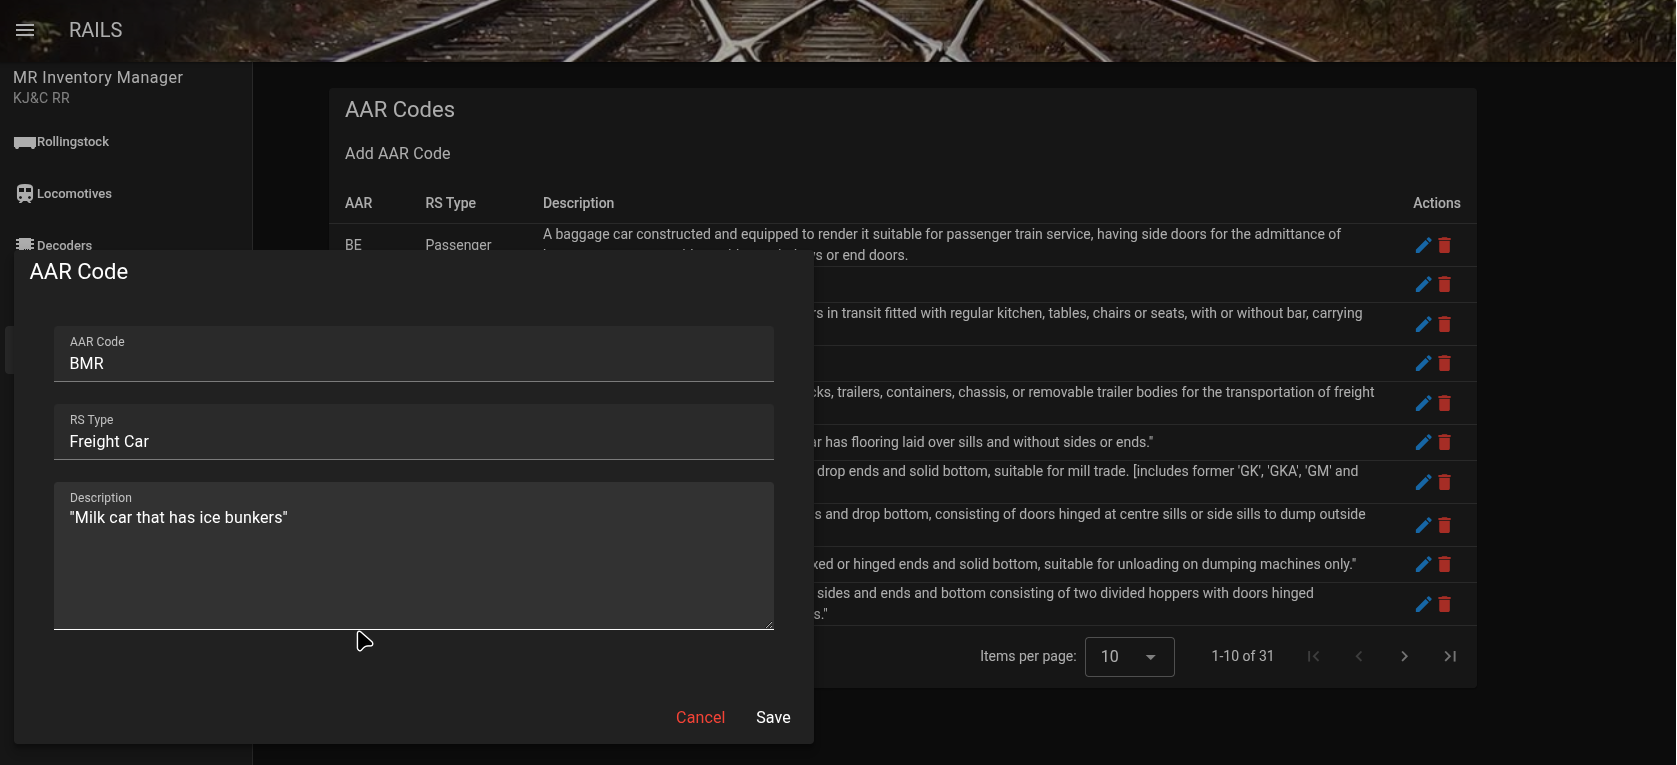
\includegraphics[width=0.85\textwidth]{./images/aar-edit.png}
    \caption{Edit AAR Code}
    \label{fig:aar-edit}
\end{figure}

\subsection{Deleting AAR Codes}

To remove a classification code from the system lookup table, click the red trash bin icon in the Actions column. A confirmation modal prompt appears requiring verification before the AAR code entry is permanently deleted. Figure \ref{fig:aar-delete} shows the deletion confirmation prompt.

\begin{figure}[H]
    \centering
    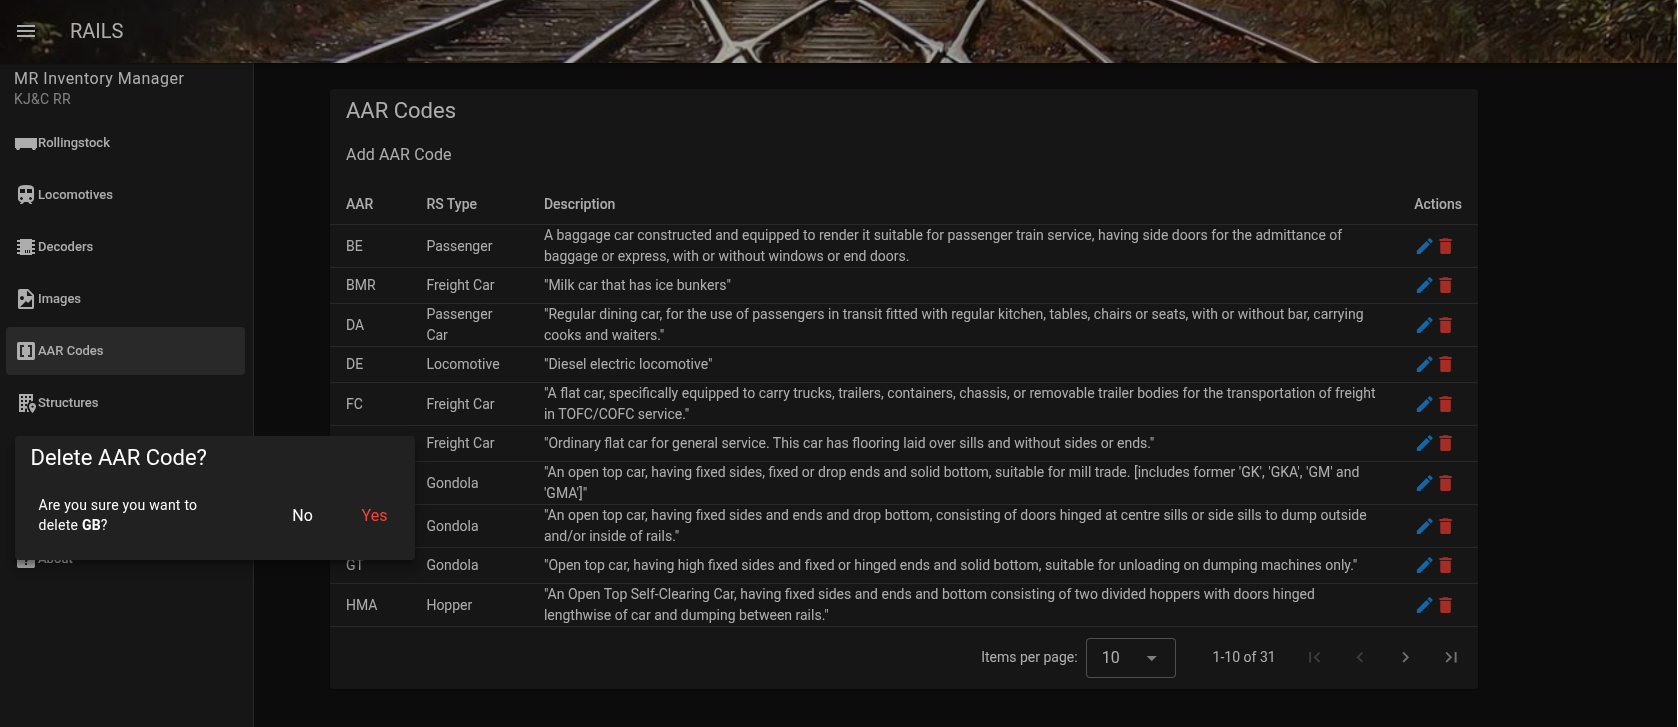
\includegraphics[width=0.85\textwidth]{./images/aar-delete.png}
    \caption{Delete AAR Code Confirmation}
    \label{fig:aar-delete}
\end{figure}
